\section{Question 2}
    Implement the k-means clustering algorithm. 
    Then, choose a 3D dataset to apply your tool and test it. 
    Explain the steps of your solution and justify your choice of the number of clusters, using graphical or numerical evidence.

\noindent\rule{\textwidth}{.5pt}

The k-means clustering algorithm is 
an expectation-maximization algorithm for unsupervised classification.
%
Output-wise, it attempts to separate the original dataset in subsets (clusters) 
that are each associated to unique label, i.e., a vector in sample space.
%
Once the algorithm is done, the samples in each group 
are assigned the values of the calculated labels;
this results in a new dataset that is a rough approximation of the original,
but that is built out of by much smaller dataset, the labels themselves.
%
Put simply, k-means attempts to reduce sample variability 
with as little information loss as possible by taking advantage of 
underlying correlations across samples. 

In further detail, the algorithm takes these steps, 
also illustrated afterwards:
%
\begin{enumerate}
    \item Initialize $k$ labels in sample space
    \item Assign each sample in the dataset to the label closest to it 
    \item Calculate the centroids of the clusters found in the previous step 
    \item If the centroids are close enough to the labels, finish the algorithm
    \item Otherwise, update the labels with the centroids values
    \item Go back to step 2
\end{enumerate}

\begin{figure}[htbp]
    \centering 
    \caption{
        Iteration of the k-means algorithm on a simple 2D dataset.
        Feature space.
        Labels are set at random from the given samples and $k=2$,
        then updated according to the clusters' averages (centroids).
        Numbers in the bubbles indicate the relevant step in the numbered list.
    }
    \label{fig:kmeans-illustration}
    \begin{tikzpicture}[> = latex]

    \def\r{.08}

    % Part 1: initialization
    \draw (1, 4) circle (.3) node {1};
    \drawDataset{black!10}{black!10}
    % Ceentroids
    \fill [red] (0.5, 1.2) circle (\r);
    \fill [blue] (1.6, 1.0) circle (\r);

    % Part 2: assigning samples according to distance
    \begin{scope}[shift={(4, 0)}]
        \draw (1, 4) circle (.3) node {2};
        \drawDataset{red!40}{blue!40}
        \draw [fill=red!40] (0.8, 0.6) circle (\r);
        % Old centroids
        \fill [red] (0.5, 1.2) circle (\r);
        \fill [blue] (1.6, 1.0) circle (\r);
        % New centroids
    \end{scope}

    % Part 3: calculate clusters' centroids 
    \begin{scope}[shift={(8, 0)}]
        \draw (1, 4) circle (.3) node {3};
        \drawDataset{red!40}{blue!40}
        \draw [fill=red!40] (0.8, 0.6) circle (\r);
        % Old centroids
        \fill [red] (0.5, 1.2) circle (\r) node (c1) {};
        \fill [blue] (1.6, 1.0) circle (\r) node (c2) {};

        % Centroids to be
        \draw (0.05, 1.625) circle (\r) node (c1-new) {};
        \draw (1.55, 0.583) circle (\r) node (c2-new) {};

        \draw [->] (c1.center) -- (c1-new.center);
        \draw [->] (c2.center) -- (c2-new.center);
    \end{scope}

    % Part 4: update centroids and clusters
    \begin{scope}[shift={(12, 0)}]
        \draw (1, 4) circle (.3) node {5};        
        \drawDataset{red!40}{blue!40}
        % Centroids
        \fill [red] (0.05, 1.625) circle (\r);
        \fill [blue] (1.55, 0.583) circle (\r);
    \end{scope}
\end{tikzpicture}
\end{figure}

I.e., k-means is template matching the data to its underlying distributions.
This overview of the algorithm introduces a number of questions that must be addressed for 
unambiguous implementation.  

First and foremost, the number $k$ of clusters/labels must be given \text{a priori}, 
despite heavily affecting the performance of the algorithm.
%
One of the possible ways of tackling this problem is 
running the algorithm for many values of $k$, which may be computationally expensive.
%
Ideally, the dataset either makes a clear suggestion of the number of clusters,
or the user has knowledge about the samples that help narrowing down the value.

Secondly, initialization of labels is not unique.
%
Although this detail usually impacts reconstruction results much less than the number of clusters,
it still plays an important role in the algorithm.
%
If a label is too far from data relative to the other labels, it risks being dropped altogether, i.e.,
no samples are assigned to it.
%
A simple method that avoids this worst case scenario, and which is used in this implementation,
is picking $k$ samples at random from the dataset as initial labels.

Thirdly, the way which distances are calculated may vary.
Usually, however, $L_2$-norm is applied, and it was preferred in this implementation.
This was also the metric used to calculate the reconstruction error across iterations.

Lastly, what defines what is ``close enough'' when deciding wheter or not 
the algorithm should stop iterating  is arbitrary.
%
Generally, the distance metric between the new centroids and the previous labels 
is compared against a ``small'' positive value $\delta_{\max}$, and if it is less than this threshold,
the algorithm ends.
%
Since what is a ``small'' threshold depends on the range of the sample space 
(a margin of $0.01$ is much tighter on attributes that range from 0-256 than 0-1),
the original dataset was centered at zero and normalized before being fed to the algorithm.
%
Additionally, it's good practice to limit the number of iterations to a set value $i_{\max}$ 
in case the centroids don't converge or take too long to do so.

With the above observations in mind, a complete flowchart of the implemented k-means algorithm
can be drawn, presented below.
%
\begin{figure}[htbp]
    \centering
    \caption{
        Implemented $k$-means algorithm.
        $\mathbf{X}^*$ denotes the zero-mean, normalized dataset,
        and $\mathbf{x}^*$ is a row from it.
        Values $r_j$ are random integers.
        Omitted: the returns of the algorithm, 
        namely the clusters $\mathcal{C}_j$, 
        labels $\mathbf{l}_j$,
        and reconstruction errors.
    }
    \label{fig:kmeans-flowchart}
    \begin{tikzpicture}[> = latex]
    \node [io] (0) at (0, 0) {
        $\mathbf{X}^*_{N\times d}$, 
        $k$, 
        $\delta_{\max}$, 
        $i_{\max}$
    };
    \node [startstop, above=1.35 of 0] (start) {Start};
    \node [process, below=1 of 0] (1) {
        $i=0$
    };
    \node [process, below=1 of 1] (2) {
        $\mathcal{R} = \{1\leq r_j\leq N\}_{1\leq j\leq k}$
    };
    \node [process, below=1 of 2] (3) {
        $\mathbf{l}_j = \mathbf{x}^*_{r_j}$, 
        $1\leq j\leq k$
    };
    \node [process, right=1 of 3] (4) {
        \begin{minipage}{5.25cm}
        \centering
            For $\mathbf{x}^*$ in $\mathbf{X}^*$:\\
            $\mathcal{C}_j \leftarrow \mathbf{x}^*,\ $
            $j = \argmin_m \lVert \mathbf{x}^* - \mathbf{l}_m\rVert_2$
        \end{minipage}
    };
    \node [process, above=1 of 4] (5) {
        $\mathbf{c}_j \leftarrow \text{Avg. of }\mathcal{C}_j$,
        $1\leq j\leq k$
    };
    \node [process, above=1 of 5] (6) {
        $\delta = \max\lVert \mathbf{l}_j-\mathbf{c}_j\rVert_2$,
        $1\leq j\leq k$
    };
    \node [decision, above=1 of 6, yshift=-.5cm] (7) {
        $\delta < \delta_{\max}$?
    };
    \node [decision, right=1 of 7, xshift=1cm] (8) {
        $i \geq i_{\max}$?
    };
    \node [process, below=0.5 of 8] (9) {
        $i \leftarrow i + 1$
    };
    \node [process, below=1 of 9] (10) {
        $\mathbf{l}_j \leftarrow \mathbf{c}_j$,
        $1\leq j\leq k$
    };
    \node [startstop, above=0.5 of 7] (stop) {Stop};

    \draw [->] (start) -- (0);
    \draw [->] (0) -- (1);
    \draw [->] (1) -- (2);
    \draw [->] (2) -- (3);
    \draw [->] (3) -- (4);
    \draw [->] (4) -- (5);
    \draw [->] (5) -- (6);
    \draw [->] (6) -- (7);
    \draw [->] (7) -- (8) node [midway, above] {no};
    \draw [->] (8) -- (9) node [midway, above right] {no};
    \draw [->] (9) -- (10);

    \draw [->] (7) -- (stop) node [midway, left] {yes};
    \draw [->] (8) |- (stop) node [midway, above] {yes};
    \draw [->] (10) |- (4);
\end{tikzpicture}
\end{figure}

To test the implementation, a small set of pictures was chosen as datasets.
These pictures, depicting either certain animals or flowers, 
come from a much bigger dataset available openly at 
\url{https://www.kaggle.com/datasets/pavansanagapati/images-dataset/data}.

The sample space corresponds to the red, green and blue values of each pixel in the image,
making it a subset of $\mathbb{R}^3$.
%
The number $k$ of clusters was decided by inspection of the figures, i.e., 
it was estimated to be equal to the number of main colors in the picture.
%
All case studies adopted a threshold $\delta_{\max}$ of $10^{-3}$, 
a maximum number of iterations $i_{\max}$ of $50$,
and had the same random seed for initialization (the integer 242104677).

Each picture tested, 
the number of clusters given to it, 
the resulting reconstruction, 
the associated reconstruction error,
and what the final clustering looked like in sample space%
\footnote{%
    A clustering always refer to the associated iteration labels \textit{before} 
    the update using the new centroids.
    E.g., if convergence is achieved in iteration 40, 
    the results presented are iteration's 39 labels and centroids.
    This is done to make sure centroids and clusters are synchronized.
}, are presented below.
%
From inspection, it is clear that the implemented k-means worked as intended,
specially for the case studies 
\texttt{cat-10.jpg},  
\texttt{flower-14.jpg},
\texttt{horse-139.jpg}, and 
\texttt{horse-170.jpg}.
%
Interestingly, cases where the algorithm did not converge within the set number of iterations
did not result in poor reconstructions, such as \texttt{cat-101.jpg} and \texttt{cat-110.jpg}.

Conversely, a small reconstruction error did not guarantee a good visual result, as in 
\texttt{horse-137.png} (note the white spots on the horse's hindleg),
\texttt{flower-6.jpg} (note how yellow tones were desaturated), and 
\texttt{flower-23.jpg} (note how a slice of the sky was highlighted).
%
Overall, however, the reconstructions are visually close to the originals,
and the reconstruction errors are small.

\begin{figure}[htbp]
    \centering
    \caption{
        Case study: \texttt{cat-10.jpg}, $k=15$.
        Original image, reconstructed image using k-means, reconstruction error,
        and clusterings in sample space.
    }
    % Top row
    \begin{subfigure}[t]{0.32\textwidth}
        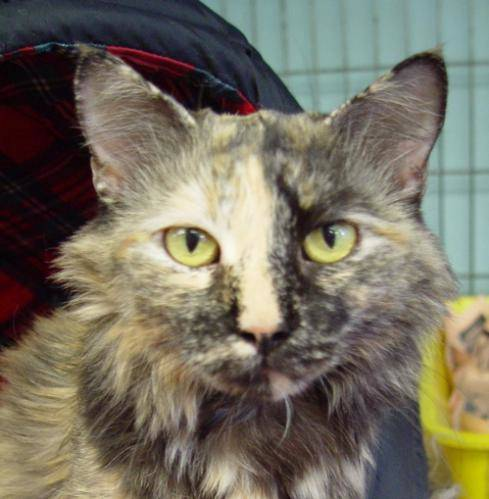
\includegraphics[width=\linewidth]{../../rust_code/data/kmeans/cat-10.jpg}
    \end{subfigure}
    \begin{subfigure}[t]{0.32\textwidth}
        
\includegraphics[width=\linewidth]{../../python_code/plots/kmeans/cat-10/reconstruction.png}
    \end{subfigure}
    \begin{subfigure}[t]{0.32\textwidth}
        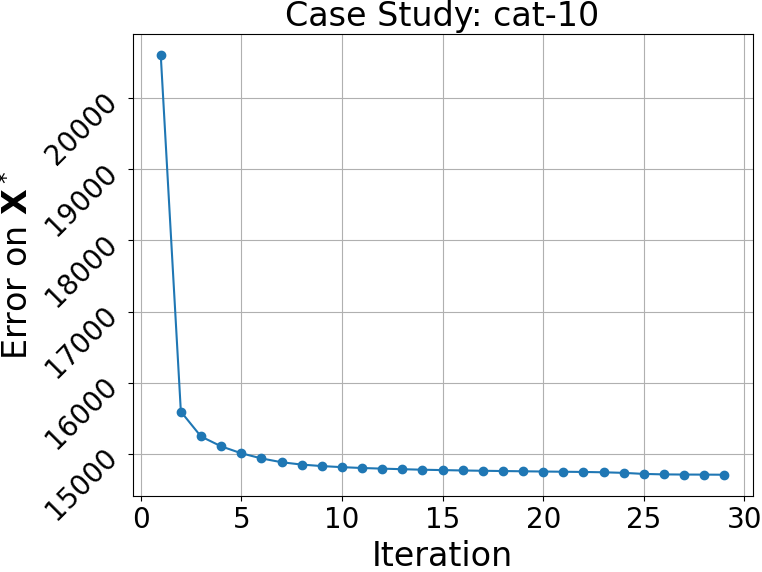
\includegraphics[width=\linewidth]{../../python_code/plots/kmeans/cat-10/elbow_curve.png}
    \end{subfigure}
    % Second row
    \begin{subfigure}[t]{0.32\textwidth}
        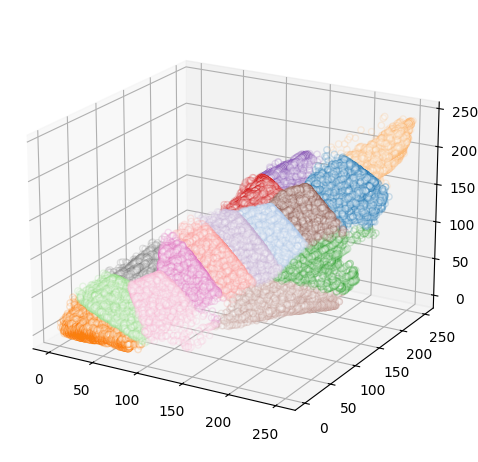
\includegraphics[width=\linewidth]{../../python_code/plots/kmeans/cat-10/clusters_elev20_azim-60.png}
    \end{subfigure}
    \begin{subfigure}[t]{0.32\textwidth}
        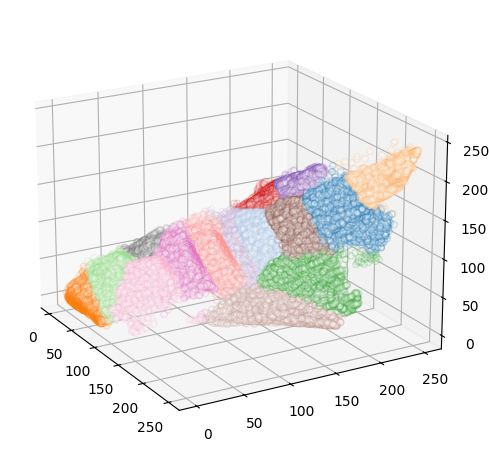
\includegraphics[width=\linewidth]{../../python_code/plots/kmeans/cat-10/clusters_elev20_azim-30.png}
    \end{subfigure}
    \begin{subfigure}[t]{0.32\textwidth}
        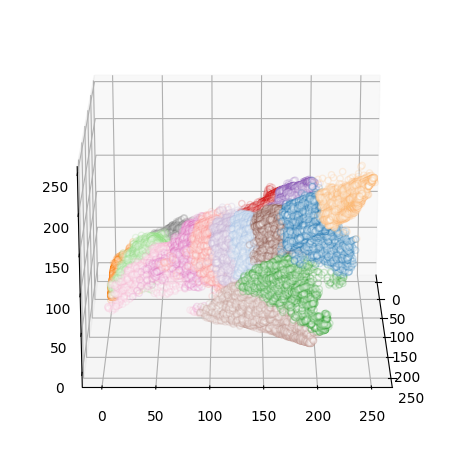
\includegraphics[width=\linewidth]{../../python_code/plots/kmeans/cat-10/clusters_elev20_azim0.png}
    \end{subfigure}
    % Third row
    \begin{subfigure}[t]{0.32\textwidth}
        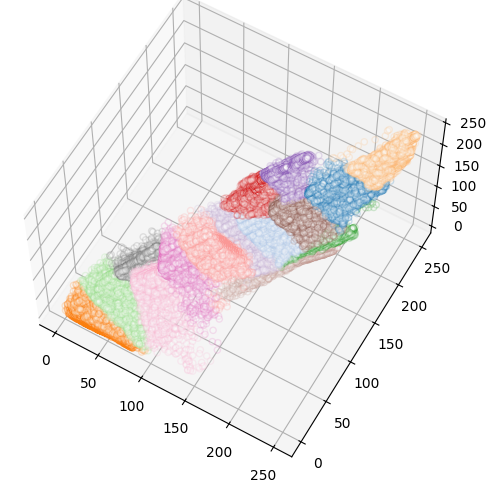
\includegraphics[width=\linewidth]{../../python_code/plots/kmeans/cat-10/clusters_elev60_azim-60.png}
    \end{subfigure}
    \begin{subfigure}[t]{0.32\textwidth}
        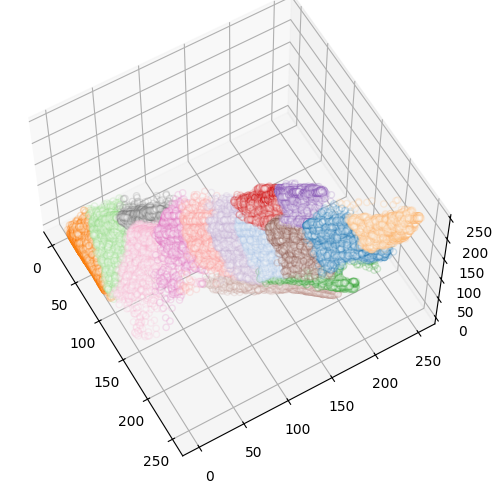
\includegraphics[width=\linewidth]{../../python_code/plots/kmeans/cat-10/clusters_elev60_azim-30.png}
    \end{subfigure}
    \begin{subfigure}[t]{0.32\textwidth}
        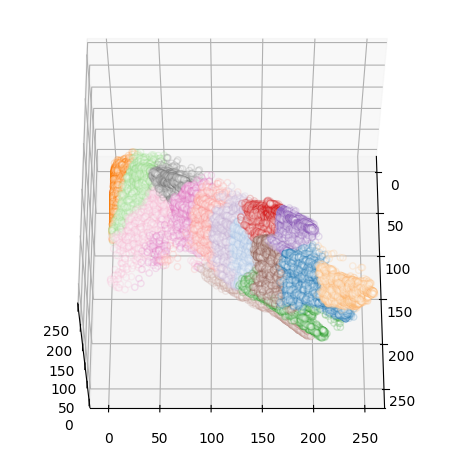
\includegraphics[width=\linewidth]{../../python_code/plots/kmeans/cat-10/clusters_elev60_azim0.png}
    \end{subfigure}
\end{figure}

\begin{figure}[htbp]
    \centering
    \caption{
        Case study: \texttt{cat-101.jpg}, $k=15$.
        Original image, reconstructed image using k-means, reconstruction error,
        and clusterings in sample space.
    }
    % Top row
    \begin{subfigure}[t]{0.32\textwidth}
        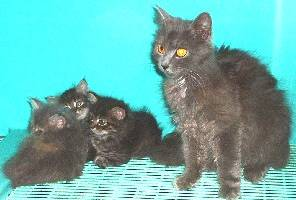
\includegraphics[width=\linewidth]{../../rust_code/data/kmeans/cat-101.jpg}
    \end{subfigure}
    \begin{subfigure}[t]{0.32\textwidth}
        
\includegraphics[width=\linewidth]{../../python_code/plots/kmeans/cat-101/reconstruction.png}
    \end{subfigure}
    \begin{subfigure}[t]{0.32\textwidth}
        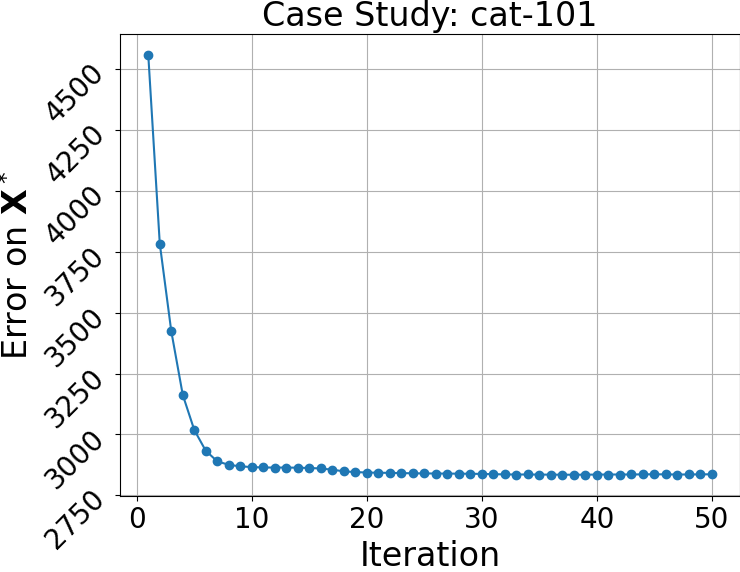
\includegraphics[width=\linewidth]{../../python_code/plots/kmeans/cat-101/elbow_curve.png}
    \end{subfigure}
    % Second row
    \begin{subfigure}[t]{0.32\textwidth}
        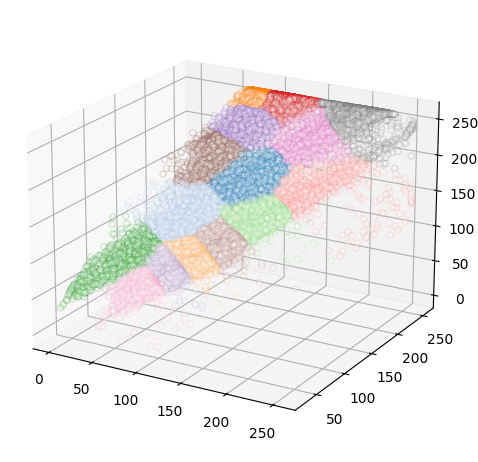
\includegraphics[width=\linewidth]{../../python_code/plots/kmeans/cat-101/clusters_elev20_azim-60.png}
    \end{subfigure}
    \begin{subfigure}[t]{0.32\textwidth}
        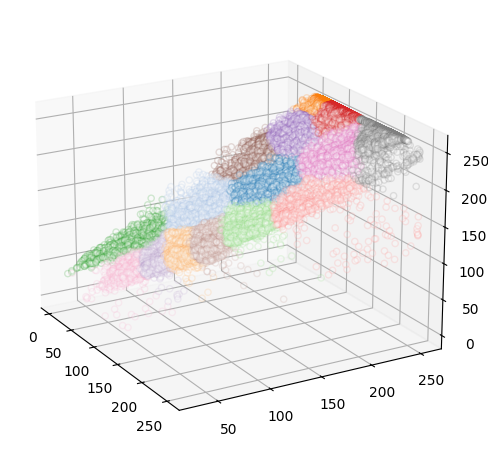
\includegraphics[width=\linewidth]{../../python_code/plots/kmeans/cat-101/clusters_elev20_azim-30.png}
    \end{subfigure}
    \begin{subfigure}[t]{0.32\textwidth}
        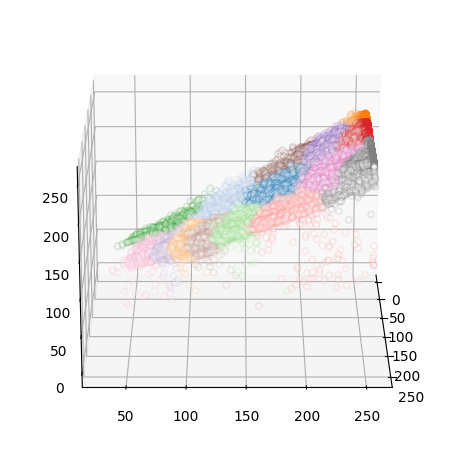
\includegraphics[width=\linewidth]{../../python_code/plots/kmeans/cat-101/clusters_elev20_azim0.png}
    \end{subfigure}
    % Third row
    \begin{subfigure}[t]{0.32\textwidth}
        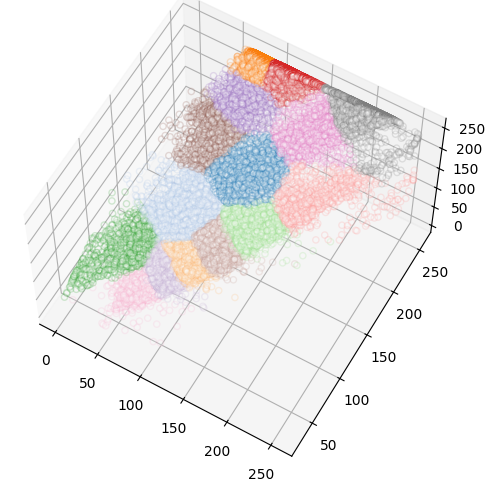
\includegraphics[width=\linewidth]{../../python_code/plots/kmeans/cat-101/clusters_elev60_azim-60.png}
    \end{subfigure}
    \begin{subfigure}[t]{0.32\textwidth}
        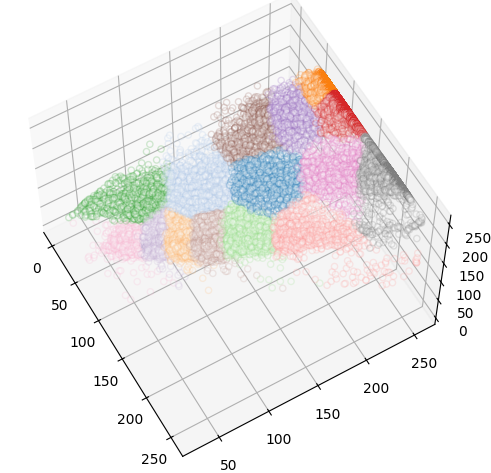
\includegraphics[width=\linewidth]{../../python_code/plots/kmeans/cat-101/clusters_elev60_azim-30.png}
    \end{subfigure}
    \begin{subfigure}[t]{0.32\textwidth}
        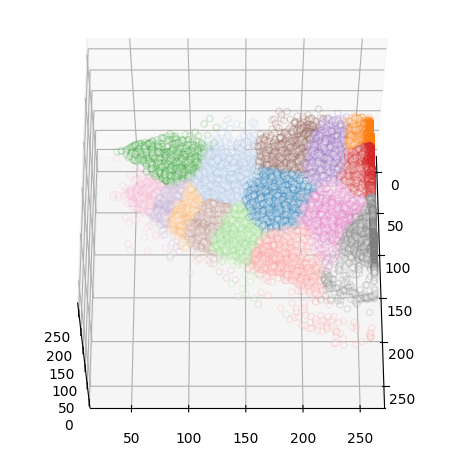
\includegraphics[width=\linewidth]{../../python_code/plots/kmeans/cat-101/clusters_elev60_azim0.png}
    \end{subfigure}
\end{figure}

\begin{figure}[htbp]
    \centering
    \caption{
        Case study: \texttt{cat-110.jpg}, $k=15$.
        Original image, reconstructed image using k-means, reconstruction error,
        and clusterings in sample space.
    }
    % Top row
    \begin{subfigure}[t]{0.32\textwidth}
        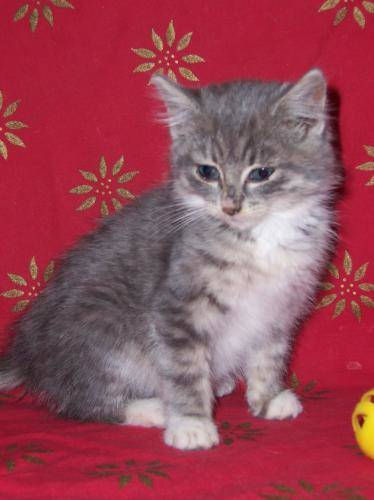
\includegraphics[width=\linewidth]{../../rust_code/data/kmeans/cat-110.jpg}
    \end{subfigure}
    \begin{subfigure}[t]{0.32\textwidth}
        
\includegraphics[width=\linewidth]{../../python_code/plots/kmeans/cat-110/reconstruction.png}
    \end{subfigure}
    \begin{subfigure}[t]{0.32\textwidth}
        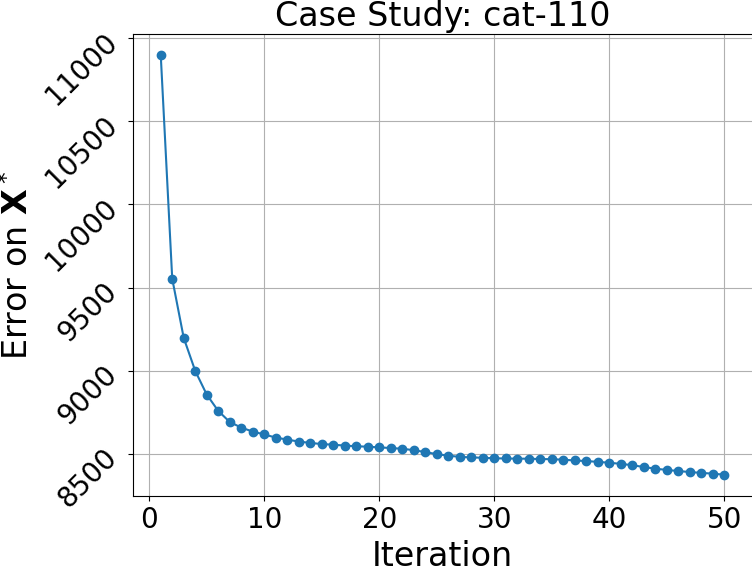
\includegraphics[width=\linewidth]{../../python_code/plots/kmeans/cat-110/elbow_curve.png}
    \end{subfigure}
    % Second row
    \begin{subfigure}[t]{0.32\textwidth}
        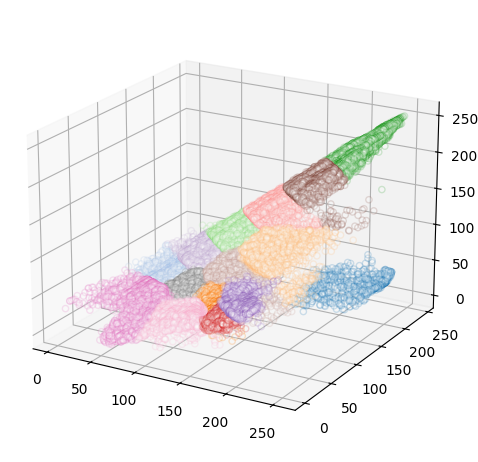
\includegraphics[width=\linewidth]{../../python_code/plots/kmeans/cat-110/clusters_elev20_azim-60.png}
    \end{subfigure}
    \begin{subfigure}[t]{0.32\textwidth}
        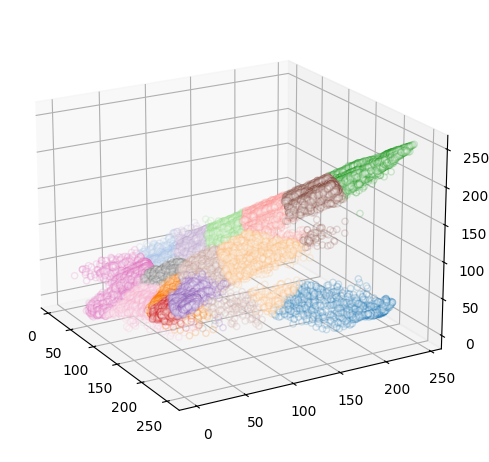
\includegraphics[width=\linewidth]{../../python_code/plots/kmeans/cat-110/clusters_elev20_azim-30.png}
    \end{subfigure}
    \begin{subfigure}[t]{0.32\textwidth}
        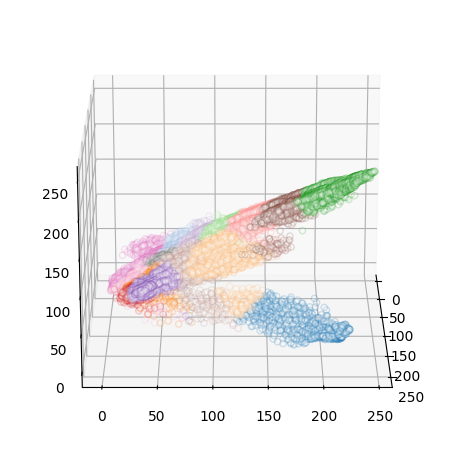
\includegraphics[width=\linewidth]{../../python_code/plots/kmeans/cat-110/clusters_elev20_azim0.png}
    \end{subfigure}
    % Third row
    \begin{subfigure}[t]{0.32\textwidth}
        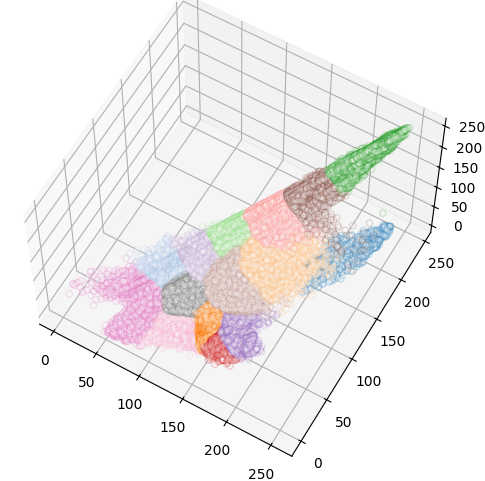
\includegraphics[width=\linewidth]{../../python_code/plots/kmeans/cat-110/clusters_elev60_azim-60.png}
    \end{subfigure}
    \begin{subfigure}[t]{0.32\textwidth}
        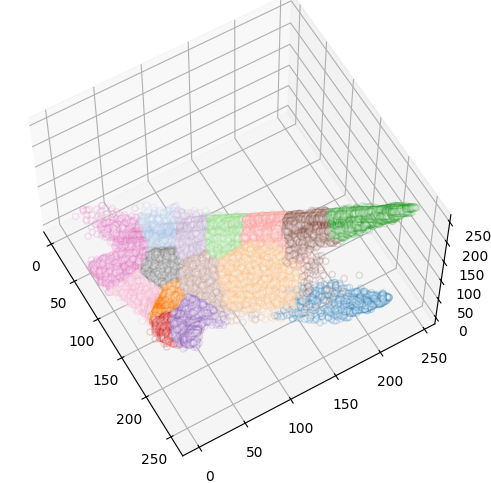
\includegraphics[width=\linewidth]{../../python_code/plots/kmeans/cat-110/clusters_elev60_azim-30.png}
    \end{subfigure}
    \begin{subfigure}[t]{0.32\textwidth}
        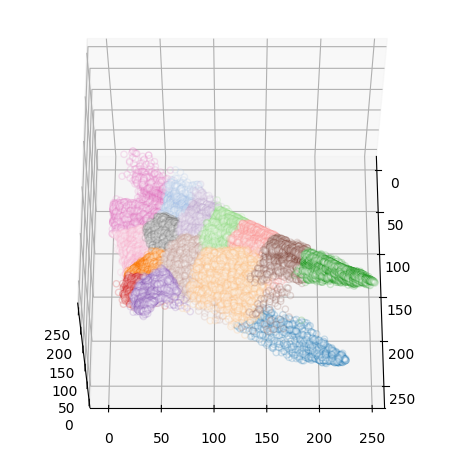
\includegraphics[width=\linewidth]{../../python_code/plots/kmeans/cat-110/clusters_elev60_azim0.png}
    \end{subfigure}
\end{figure}

\begin{figure}[htbp]
    \centering
    \caption{
        Case study: \texttt{flower-6.jpg}, $k=10$.
        Original image, reconstructed image using k-means, reconstruction error,
        and clusterings in sample space.
    }
    % Top row
    \begin{subfigure}[t]{0.32\textwidth}
        
\includegraphics[width=\linewidth]{../../rust_code/data/kmeans/flower-6.jpg}
    \end{subfigure}
    \begin{subfigure}[t]{0.32\textwidth}
        
\includegraphics[width=\linewidth]{../../python_code/plots/kmeans/flower-6/reconstruction.png}
    \end{subfigure}
    \begin{subfigure}[t]{0.32\textwidth}
        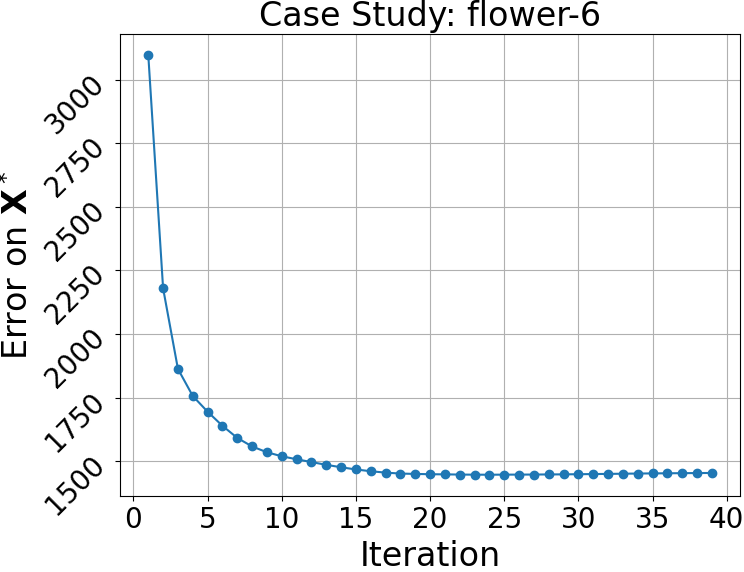
\includegraphics[width=\linewidth]{../../python_code/plots/kmeans/flower-6/elbow_curve.png}
    \end{subfigure}
    % Second row
    \begin{subfigure}[t]{0.32\textwidth}
        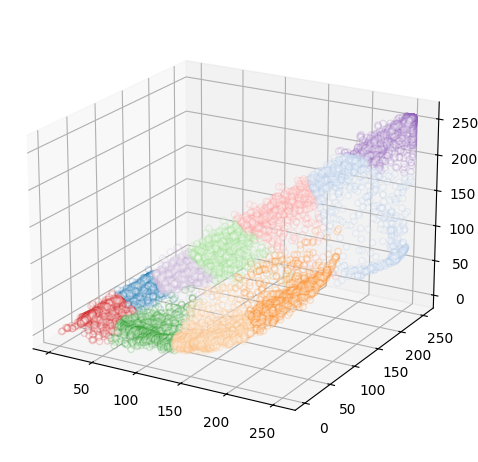
\includegraphics[width=\linewidth]{../../python_code/plots/kmeans/flower-6/clusters_elev20_azim-60.png}
    \end{subfigure}
    \begin{subfigure}[t]{0.32\textwidth}
        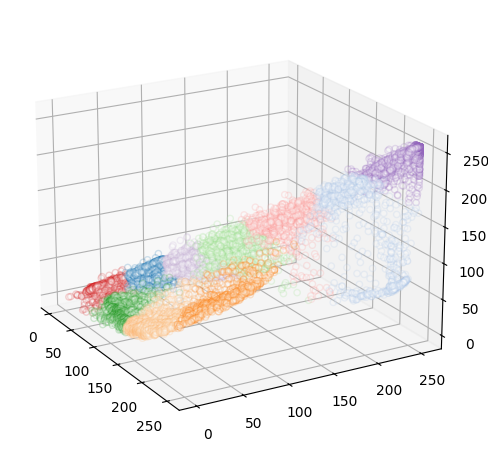
\includegraphics[width=\linewidth]{../../python_code/plots/kmeans/flower-6/clusters_elev20_azim-30.png}
    \end{subfigure}
    \begin{subfigure}[t]{0.32\textwidth}
        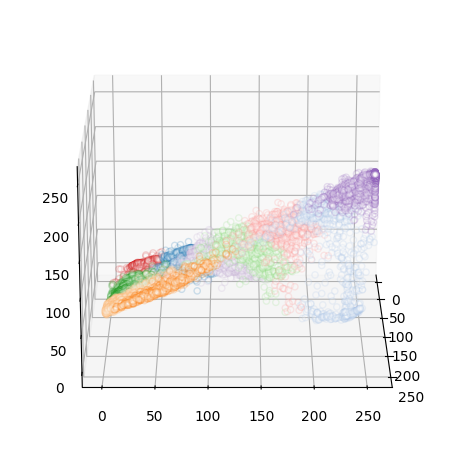
\includegraphics[width=\linewidth]{../../python_code/plots/kmeans/flower-6/clusters_elev20_azim0.png}
    \end{subfigure}
    % Third row
    \begin{subfigure}[t]{0.32\textwidth}
        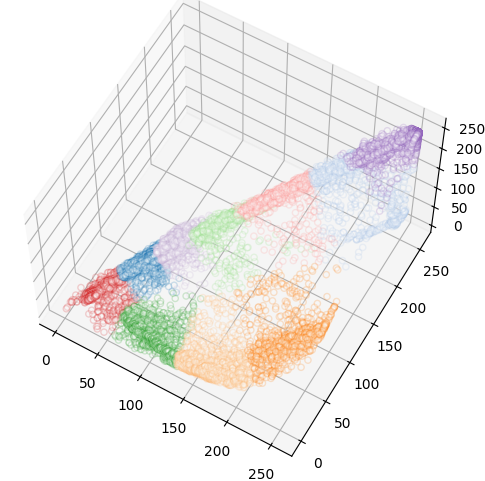
\includegraphics[width=\linewidth]{../../python_code/plots/kmeans/flower-6/clusters_elev60_azim-60.png}
    \end{subfigure}
    \begin{subfigure}[t]{0.32\textwidth}
        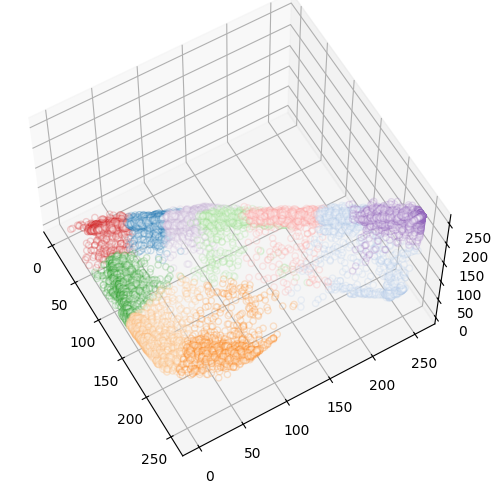
\includegraphics[width=\linewidth]{../../python_code/plots/kmeans/flower-6/clusters_elev60_azim-30.png}
    \end{subfigure}
    \begin{subfigure}[t]{0.32\textwidth}
        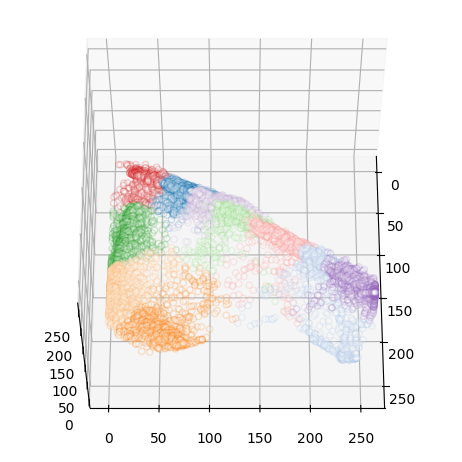
\includegraphics[width=\linewidth]{../../python_code/plots/kmeans/flower-6/clusters_elev60_azim0.png}
    \end{subfigure}
\end{figure}

\begin{figure}[htbp]
    \centering
    \caption{
        Case study: \texttt{flower-14.jpg}, $k=10$.
        Original image, reconstructed image using k-means, reconstruction error,
        and clusterings in sample space.
    }
    % Top row
    \begin{subfigure}[t]{0.32\textwidth}
        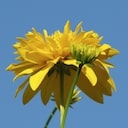
\includegraphics[width=\linewidth]{../../rust_code/data/kmeans/flower-14.jpg}
    \end{subfigure}
    \begin{subfigure}[t]{0.32\textwidth}
        
\includegraphics[width=\linewidth]{../../python_code/plots/kmeans/flower-14/reconstruction.png}
    \end{subfigure}
    \begin{subfigure}[t]{0.32\textwidth}
        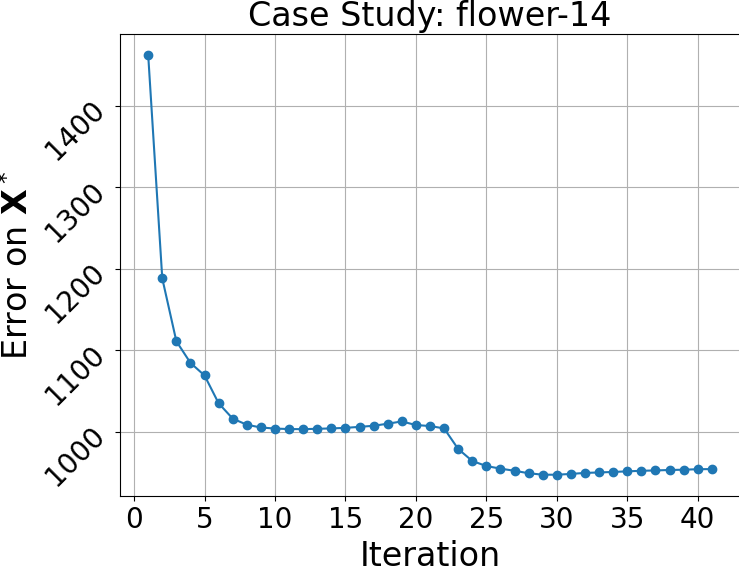
\includegraphics[width=\linewidth]{../../python_code/plots/kmeans/flower-14/elbow_curve.png}
    \end{subfigure}
    % Second row
    \begin{subfigure}[t]{0.32\textwidth}
        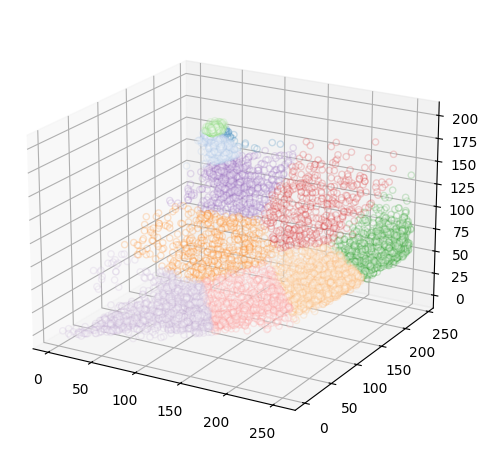
\includegraphics[width=\linewidth]{../../python_code/plots/kmeans/flower-14/clusters_elev20_azim-60.png}
    \end{subfigure}
    \begin{subfigure}[t]{0.32\textwidth}
        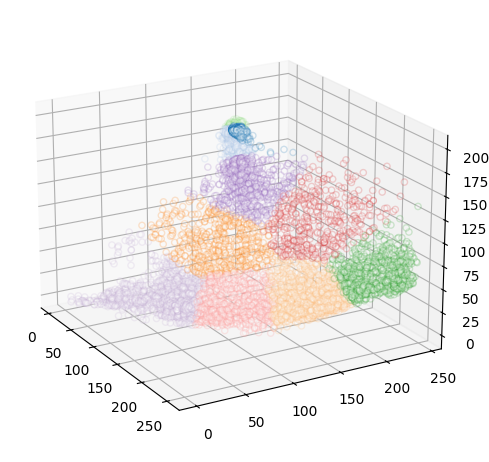
\includegraphics[width=\linewidth]{../../python_code/plots/kmeans/flower-14/clusters_elev20_azim-30.png}
    \end{subfigure}
    \begin{subfigure}[t]{0.32\textwidth}
        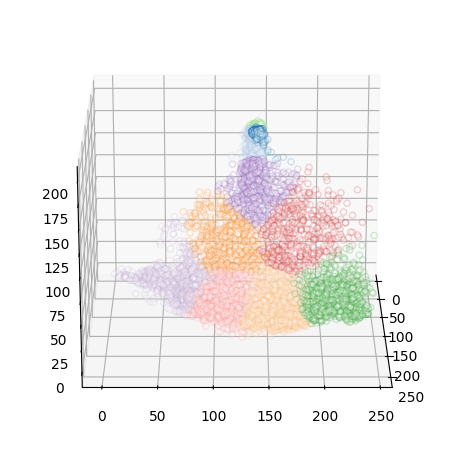
\includegraphics[width=\linewidth]{../../python_code/plots/kmeans/flower-14/clusters_elev20_azim0.png}
    \end{subfigure}
    % Third row
    \begin{subfigure}[t]{0.32\textwidth}
        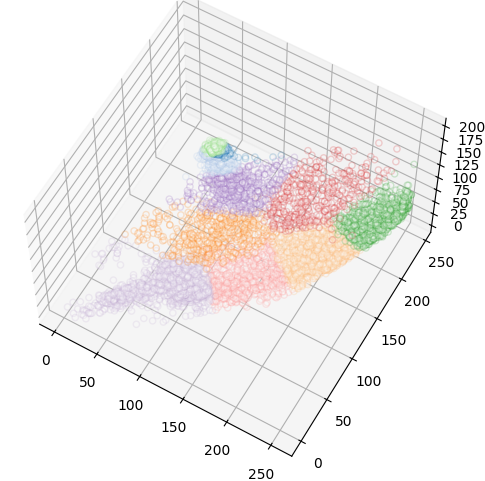
\includegraphics[width=\linewidth]{../../python_code/plots/kmeans/flower-14/clusters_elev60_azim-60.png}
    \end{subfigure}
    \begin{subfigure}[t]{0.32\textwidth}
        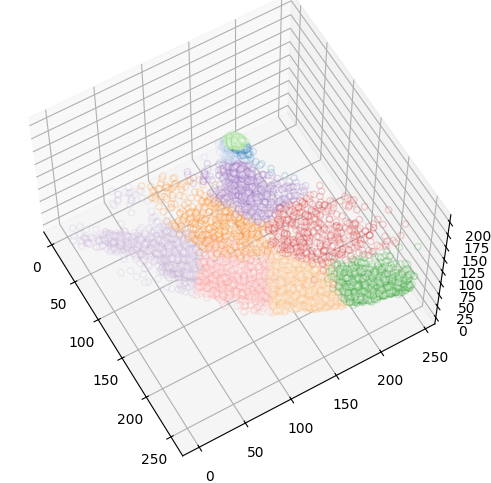
\includegraphics[width=\linewidth]{../../python_code/plots/kmeans/flower-14/clusters_elev60_azim-30.png}
    \end{subfigure}
    \begin{subfigure}[t]{0.32\textwidth}
        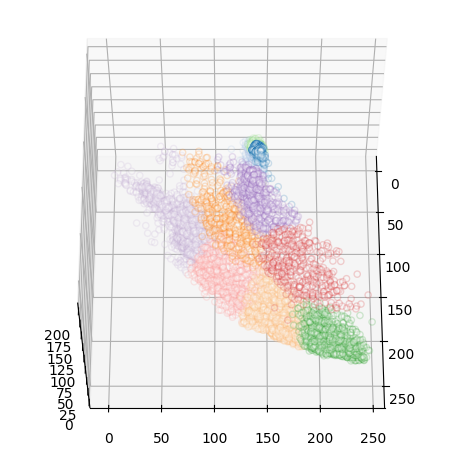
\includegraphics[width=\linewidth]{../../python_code/plots/kmeans/flower-14/clusters_elev60_azim0.png}
    \end{subfigure}
\end{figure}

\begin{figure}[htbp]
    \centering
    \caption{
        Case study: \texttt{flower-23.jpg}, $k=10$.
        Original image, reconstructed image using k-means, reconstruction error,
        and clusterings in sample space.
    }
    % Top row
    \begin{subfigure}[t]{0.32\textwidth}
        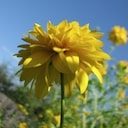
\includegraphics[width=\linewidth]{../../rust_code/data/kmeans/flower-23.jpg}
    \end{subfigure}
    \begin{subfigure}[t]{0.32\textwidth}
        
\includegraphics[width=\linewidth]{../../python_code/plots/kmeans/flower-23/reconstruction.png}
    \end{subfigure}
    \begin{subfigure}[t]{0.32\textwidth}
        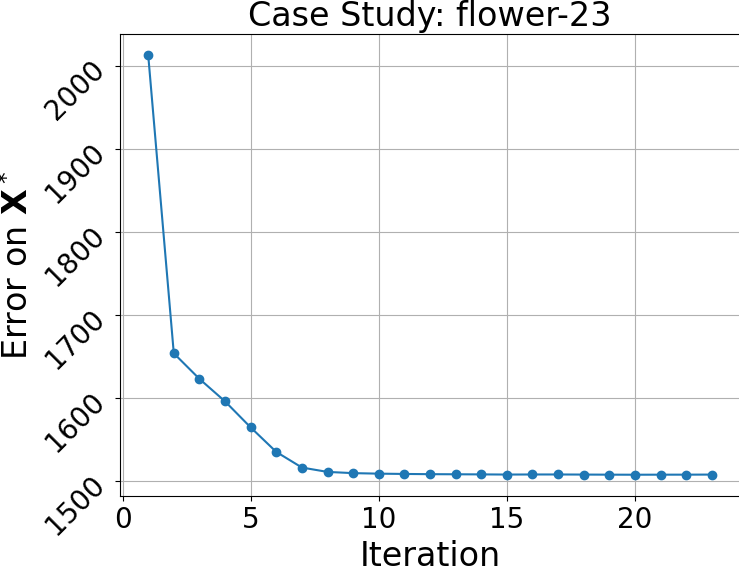
\includegraphics[width=\linewidth]{../../python_code/plots/kmeans/flower-23/elbow_curve.png}
    \end{subfigure}
    % Second row
    \begin{subfigure}[t]{0.32\textwidth}
        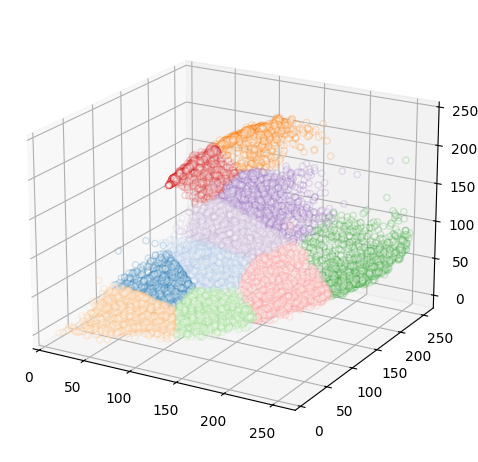
\includegraphics[width=\linewidth]{../../python_code/plots/kmeans/flower-23/clusters_elev20_azim-60.png}
    \end{subfigure}
    \begin{subfigure}[t]{0.32\textwidth}
        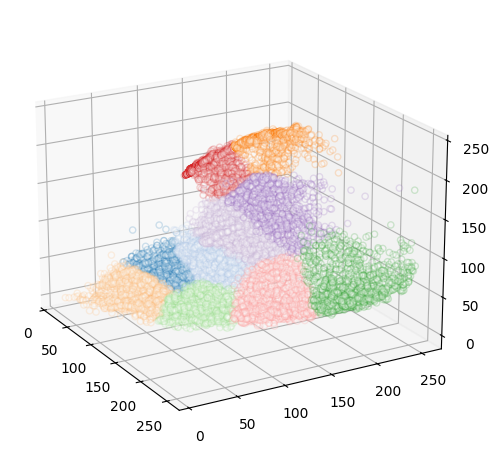
\includegraphics[width=\linewidth]{../../python_code/plots/kmeans/flower-23/clusters_elev20_azim-30.png}
    \end{subfigure}
    \begin{subfigure}[t]{0.32\textwidth}
        \includegraphics[width=\linewidth]{../../python_code/plots/kmeans/flower-23/clusters_elev20_azim0.png}
    \end{subfigure}
    % Third row
    \begin{subfigure}[t]{0.32\textwidth}
        \includegraphics[width=\linewidth]{../../python_code/plots/kmeans/flower-23/clusters_elev60_azim-60.png}
    \end{subfigure}
    \begin{subfigure}[t]{0.32\textwidth}
        \includegraphics[width=\linewidth]{../../python_code/plots/kmeans/flower-23/clusters_elev60_azim-30.png}
    \end{subfigure}
    \begin{subfigure}[t]{0.32\textwidth}
        \includegraphics[width=\linewidth]{../../python_code/plots/kmeans/flower-23/clusters_elev60_azim0.png}
    \end{subfigure}
\end{figure}

\begin{figure}[htbp]
    \centering
    \caption{
        Case study: \texttt{horse-137.jpg}, $k=10$.
        Original image, reconstructed image using k-means, reconstruction error,
        and clusterings in sample space.
    }
    % Top row
    \begin{subfigure}[t]{0.32\textwidth}
        \includegraphics[width=\linewidth]{../../rust_code/data/kmeans/horse-137.jpg}
    \end{subfigure}
    \begin{subfigure}[t]{0.32\textwidth}
        \includegraphics[width=\linewidth]{../../python_code/plots/kmeans/horse-137/reconstruction.png}
    \end{subfigure}
    \begin{subfigure}[t]{0.32\textwidth}
        \includegraphics[width=\linewidth]{../../python_code/plots/kmeans/horse-137/elbow_curve.png}
    \end{subfigure}
    % Second row
    \begin{subfigure}[t]{0.32\textwidth}
        \includegraphics[width=\linewidth]{../../python_code/plots/kmeans/horse-137/clusters_elev20_azim-60.png}
    \end{subfigure}
    \begin{subfigure}[t]{0.32\textwidth}
        \includegraphics[width=\linewidth]{../../python_code/plots/kmeans/horse-137/clusters_elev20_azim-30.png}
    \end{subfigure}
    \begin{subfigure}[t]{0.32\textwidth}
        \includegraphics[width=\linewidth]{../../python_code/plots/kmeans/horse-137/clusters_elev20_azim0.png}
    \end{subfigure}
    % Third row
    \begin{subfigure}[t]{0.32\textwidth}
        \includegraphics[width=\linewidth]{../../python_code/plots/kmeans/horse-137/clusters_elev60_azim-60.png}
    \end{subfigure}
    \begin{subfigure}[t]{0.32\textwidth}
        \includegraphics[width=\linewidth]{../../python_code/plots/kmeans/horse-137/clusters_elev60_azim-30.png}
    \end{subfigure}
    \begin{subfigure}[t]{0.32\textwidth}
        \includegraphics[width=\linewidth]{../../python_code/plots/kmeans/horse-137/clusters_elev60_azim0.png}
    \end{subfigure}
\end{figure}

\begin{figure}[htbp]
    \centering
    \caption{
        Case study: \texttt{horse-139.jpg}, $k=15$.
        Original image, reconstructed image using k-means, reconstruction error,
        and clusterings in sample space.
    }
    % Top row
    \begin{subfigure}[t]{0.32\textwidth}
        \includegraphics[width=\linewidth]{../../rust_code/data/kmeans/horse-139.jpg}
    \end{subfigure}
    \begin{subfigure}[t]{0.32\textwidth}
        \includegraphics[width=\linewidth]{../../python_code/plots/kmeans/horse-139/reconstruction.png}
    \end{subfigure}
    \begin{subfigure}[t]{0.32\textwidth}
        \includegraphics[width=\linewidth]{../../python_code/plots/kmeans/horse-139/elbow_curve.png}
    \end{subfigure}
    % Second row
    \begin{subfigure}[t]{0.32\textwidth}
        \includegraphics[width=\linewidth]{../../python_code/plots/kmeans/horse-139/clusters_elev20_azim-60.png}
    \end{subfigure}
    \begin{subfigure}[t]{0.32\textwidth}
        \includegraphics[width=\linewidth]{../../python_code/plots/kmeans/horse-139/clusters_elev20_azim-30.png}
    \end{subfigure}
    \begin{subfigure}[t]{0.32\textwidth}
        \includegraphics[width=\linewidth]{../../python_code/plots/kmeans/horse-139/clusters_elev20_azim0.png}
    \end{subfigure}
    % Third row
    \begin{subfigure}[t]{0.32\textwidth}
        \includegraphics[width=\linewidth]{../../python_code/plots/kmeans/horse-139/clusters_elev60_azim-60.png}
    \end{subfigure}
    \begin{subfigure}[t]{0.32\textwidth}
        \includegraphics[width=\linewidth]{../../python_code/plots/kmeans/horse-139/clusters_elev60_azim-30.png}
    \end{subfigure}
    \begin{subfigure}[t]{0.32\textwidth}
        \includegraphics[width=\linewidth]{../../python_code/plots/kmeans/horse-139/clusters_elev60_azim0.png}
    \end{subfigure}
\end{figure}

\begin{figure}[htbp]
    \centering
    \caption{
        Case study: \texttt{horse-170.jpg}, $k=15$.
        Original image, reconstructed image using k-means, reconstruction error,
        and clusterings in sample space.
    }
    % Top row
    \begin{subfigure}[t]{0.32\textwidth}
        \includegraphics[width=\linewidth]{../../rust_code/data/kmeans/horse-170.jpg}
    \end{subfigure}
    \begin{subfigure}[t]{0.32\textwidth}
        \includegraphics[width=\linewidth]{../../python_code/plots/kmeans/horse-170/reconstruction.png}
    \end{subfigure}
    \begin{subfigure}[t]{0.32\textwidth}
        \includegraphics[width=\linewidth]{../../python_code/plots/kmeans/horse-170/elbow_curve.png}
    \end{subfigure}
    % Second row
    \begin{subfigure}[t]{0.32\textwidth}
        \includegraphics[width=\linewidth]{../../python_code/plots/kmeans/horse-170/clusters_elev20_azim-60.png}
    \end{subfigure}
    \begin{subfigure}[t]{0.32\textwidth}
        \includegraphics[width=\linewidth]{../../python_code/plots/kmeans/horse-170/clusters_elev20_azim-30.png}
    \end{subfigure}
    \begin{subfigure}[t]{0.32\textwidth}
        \includegraphics[width=\linewidth]{../../python_code/plots/kmeans/horse-170/clusters_elev20_azim0.png}
    \end{subfigure}
    % Third row
    \begin{subfigure}[t]{0.32\textwidth}
        \includegraphics[width=\linewidth]{../../python_code/plots/kmeans/horse-170/clusters_elev60_azim-60.png}
    \end{subfigure}
    \begin{subfigure}[t]{0.32\textwidth}
        \includegraphics[width=\linewidth]{../../python_code/plots/kmeans/horse-170/clusters_elev60_azim-30.png}
    \end{subfigure}
    \begin{subfigure}[t]{0.32\textwidth}
        \includegraphics[width=\linewidth]{../../python_code/plots/kmeans/horse-170/clusters_elev60_azim0.png}
    \end{subfigure}
\end{figure}
    